\documentclass{article}
\usepackage{graphicx}
\usepackage[margin=1.5cm]{geometry}
\usepackage{amsmath}

\begin{document}

\title{Warm-Up 17}
\author{Prof. Jordan C. Hanson}

\maketitle

\section{The US Census, 2020}

\begin{enumerate}
\item The US Census is conducted every 10 years, and 2020 happens to be a census year.  Consider Fig. \ref{fig:population}.  (a) By how many people has the population of Los Angeles County grown since 2010?  (b) What is the percent change?  (c) What will the population of Los Angeles County be in 2030, assuming the same trend holds?  (d) The US Constitution prescribes that the ``whole number of persons'' living in each State be counted, and Census workers try to meet this goal as best they can.  However, it's not always possible to count every last whole person in a place like Los Angeles.  Describe a method using statistical sampling that could give you an accurate estimate of the \textit{percent growth} in population.
\begin{figure}[ht]
\centering
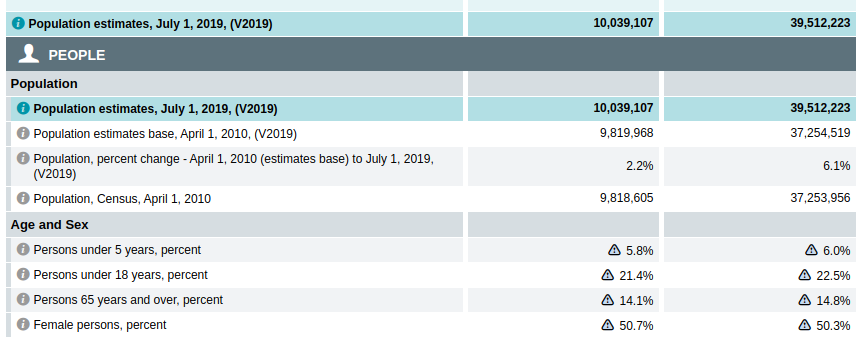
\includegraphics[width=0.65\textwidth]{population.png}
\caption{\label{fig:population} US Census data from 2019 for Los Angeles County, California.}
\end{figure}
\item Suppose someone is measuring GPA data from Whittier College first-years, and makes the following claim: ``The GPA distribution follows a standard-normal distribution.  Therefore, we can predict the fraction of students that will have a GPA 2 standard deviations below the mean GPA.''  (a) Call this hypothesis the \textit{null hypothesis} and any alternative the \textit{alternative hypothesis.}  Based on Fig. \ref{fig:gpa}, do you reject the null hypothesis or accept it?  (b) Construct a statistical claim that accurately describes the GPA distribution.
\begin{figure}[hb]
\centering
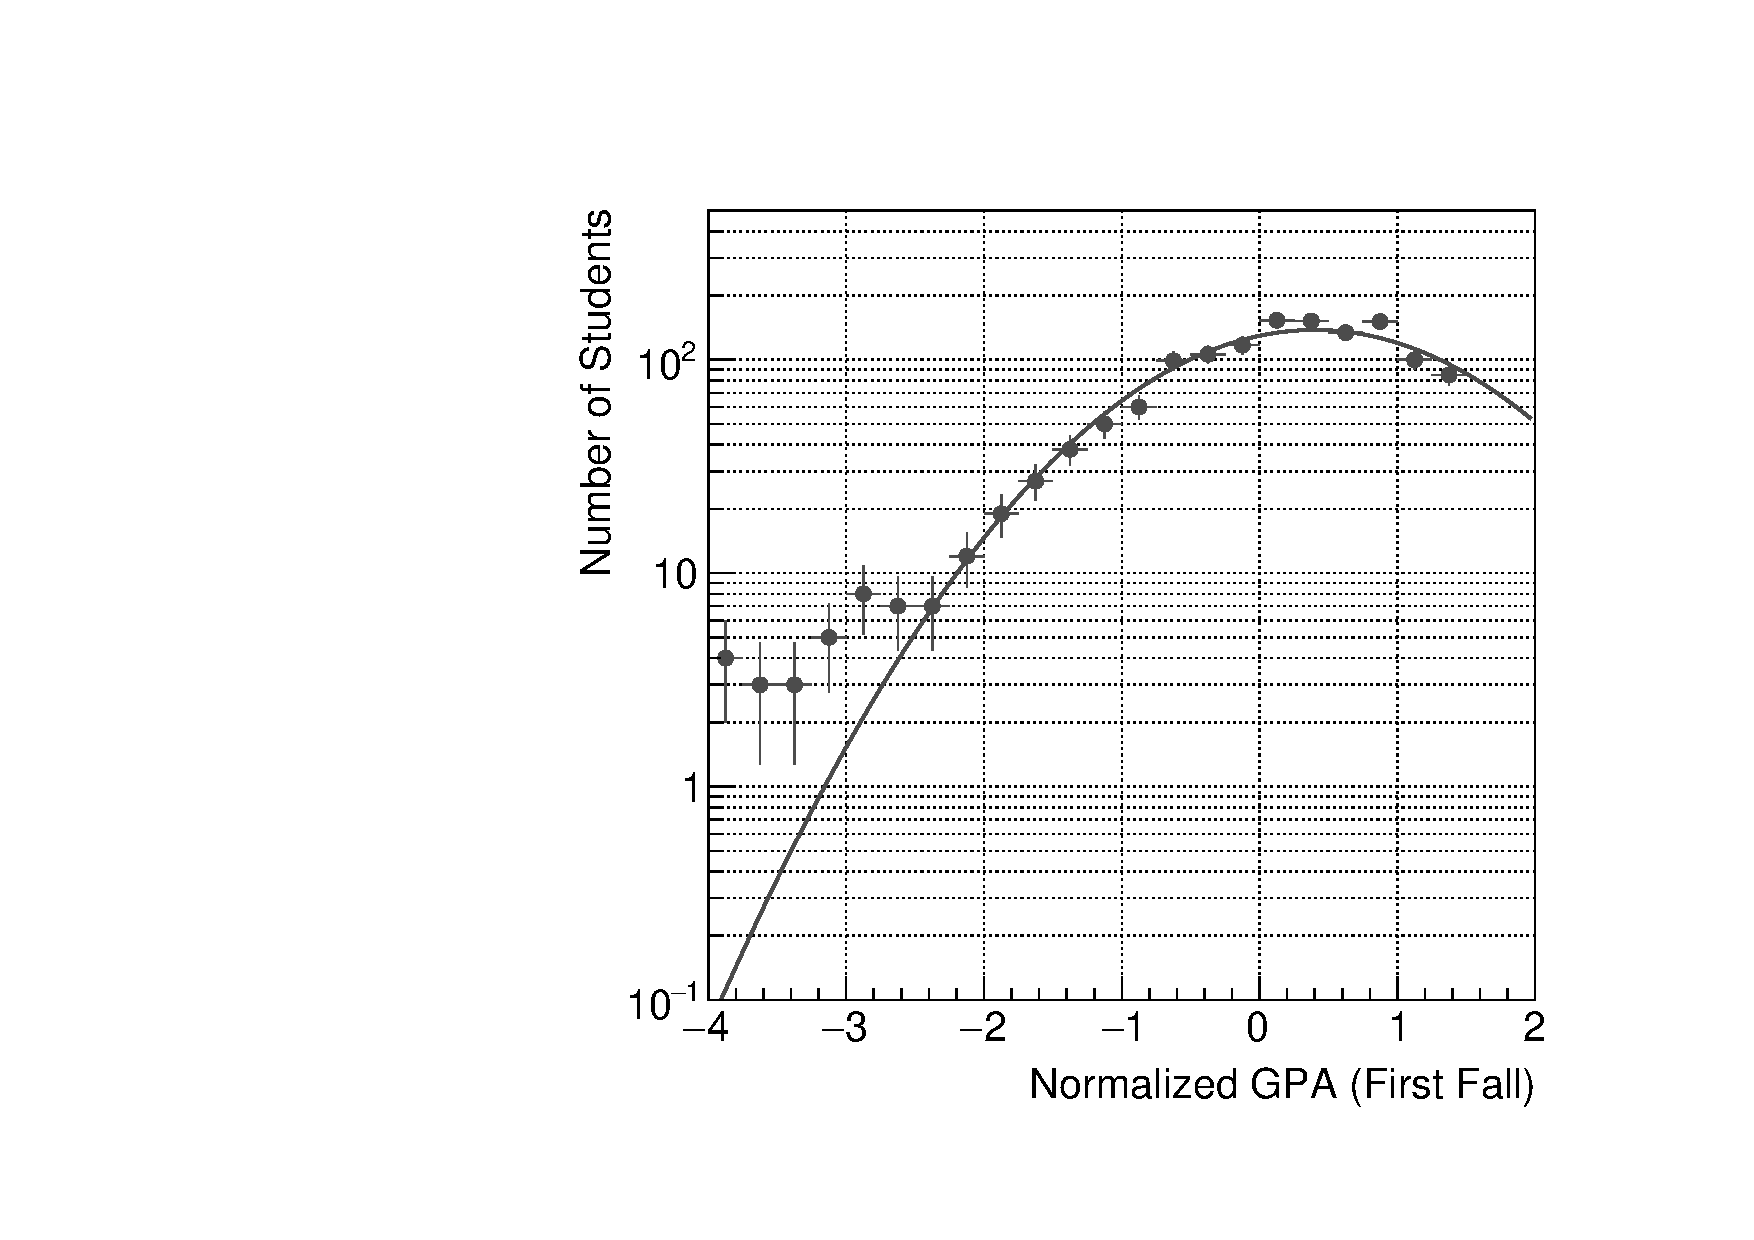
\includegraphics[width=0.35\textwidth]{Nov15_plot3.pdf}
\caption{\label{fig:gpa} Z-score for Whittier College students' GPA in their first fall semester as first-years.}
\end{figure}
\end{enumerate}

\end{document}